\section{Topology optimization of a motorcycle frame}
\label{sec:motorcycle_frame}

\subsection{Requests}
\label{subsec:mf_requests}

The goal of this section is to perform a topology optimization of a motorcycle frame shown in Figure \ref{fig:motorcycle_frame}, minimizing the compliance $C$ by acting on the cross-sectional areas of the beams.
A maximum volume constraint $V_{structure} \le V_0$ is also imposed.

\begin{figure}[H]
    \centering
    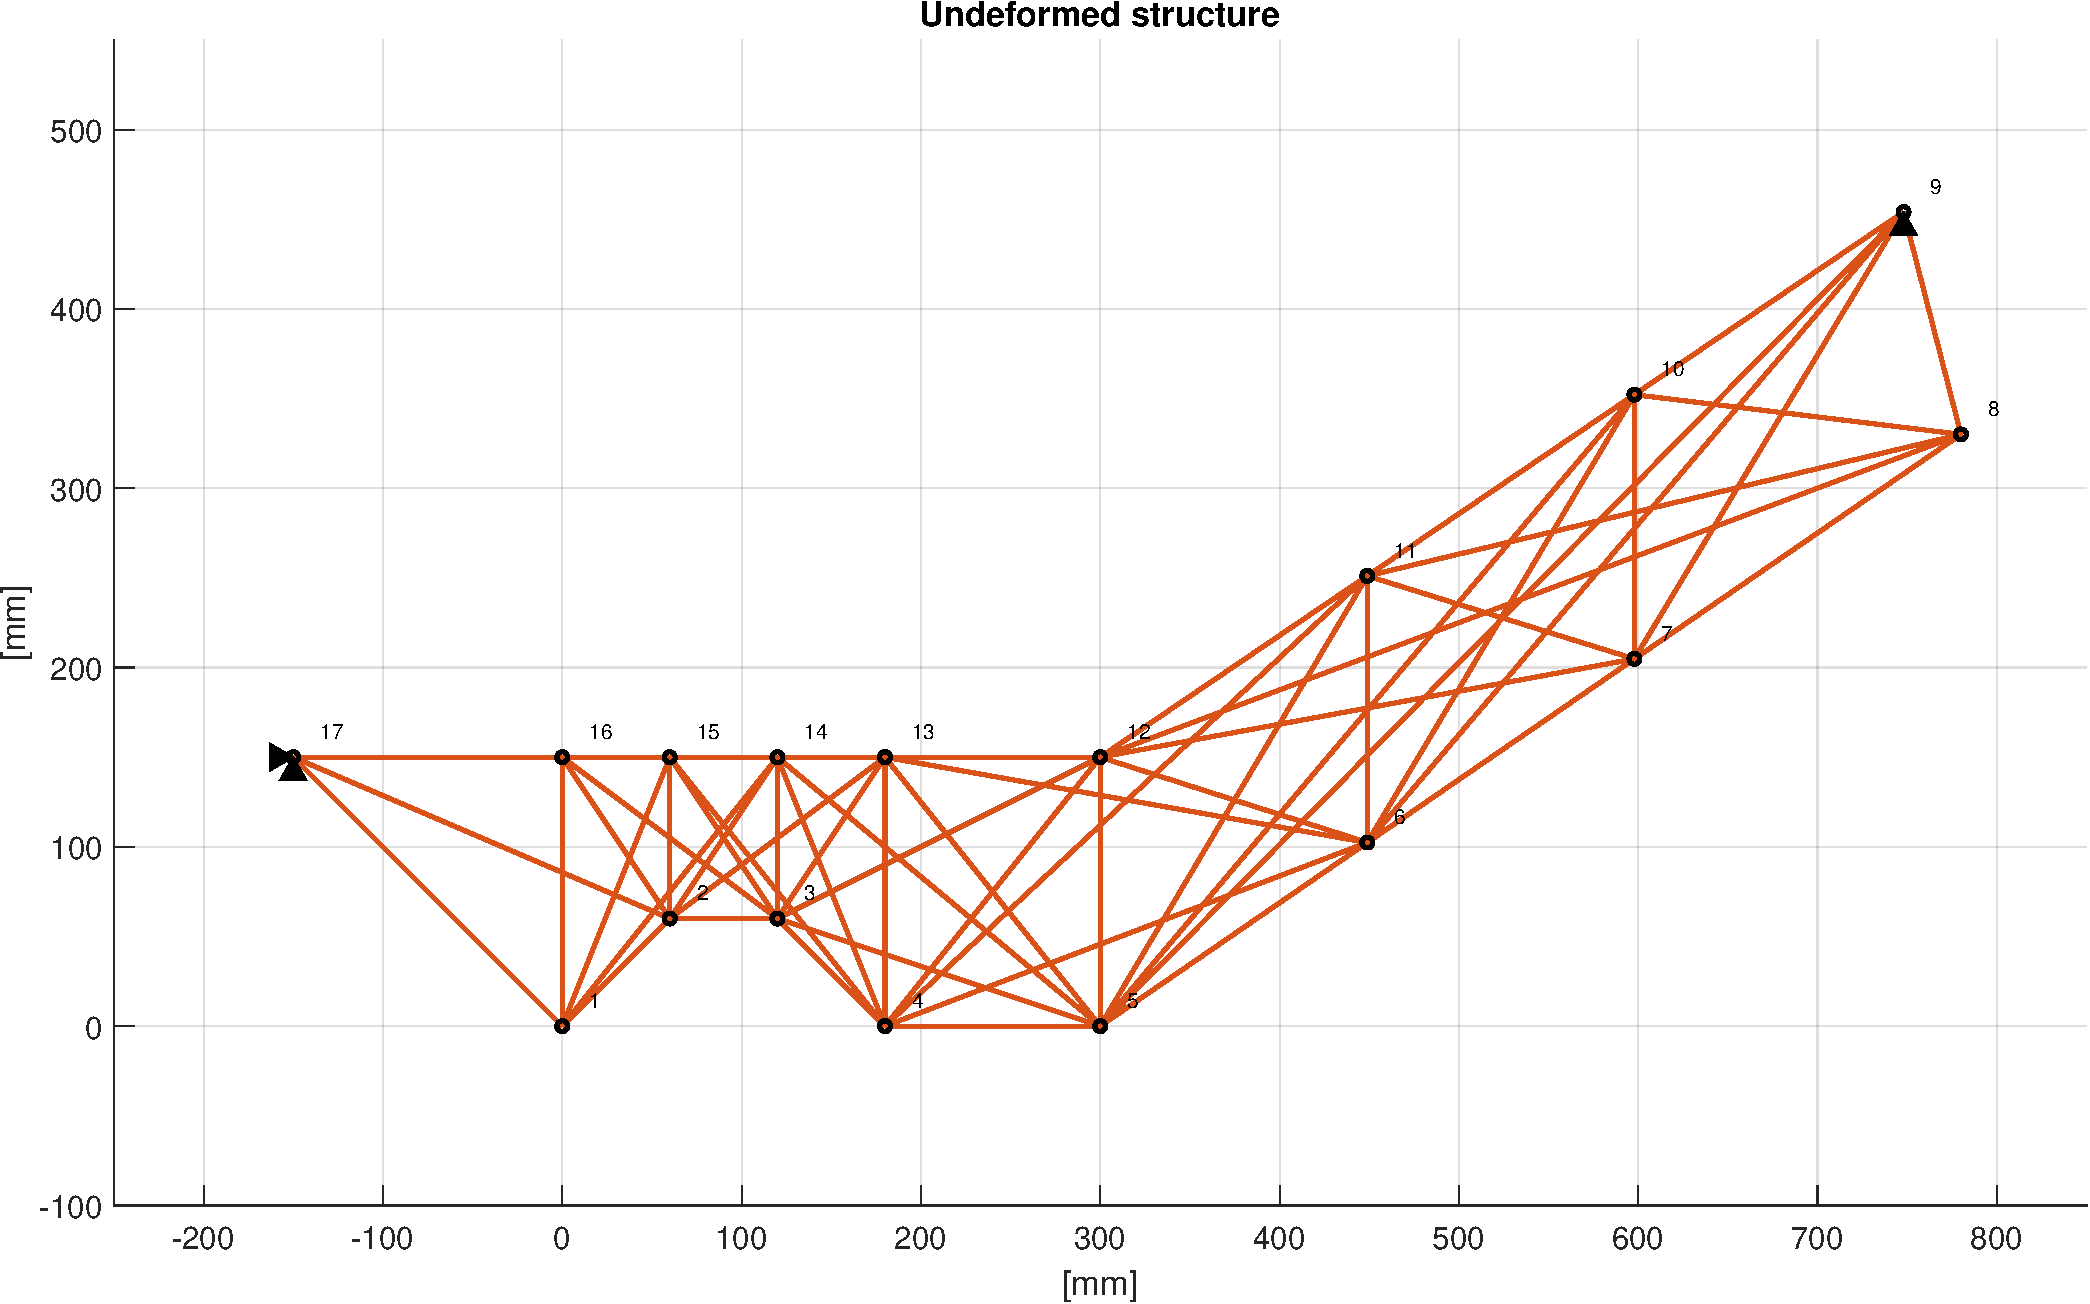
\includegraphics[width=0.8\textwidth]{img/MATLAB/motorcycle_frame/undeformed_structure.pdf}
    \caption{Unloaded motorcycle frame to be optimized}
    \label{fig:motorcycle_frame}
\end{figure}

As can be observed, the structure is composed of $N_{nodes} = 17$ nodes and $N_{beams} = 55$ beams.
Node indexes are indicated in the figure by the numbers reported besides each node, while the black triangles connected to some nodes represent the applied constraints.
In particular, vertical constrains are imposed on nodes ${9, 17}$, while horizontal constrains are also imposed on node ${17}$.

For the case at hand, we suppose to optimize the structure simultaneously for the two most severe load conditions of such frame, which are braking and acceleration.
Data for the two load cases are reported in Table \ref{tab:load_braking} and Table \ref{tab:load_acceleration}, respectively.

\begin{table}[H]
    \centering

    \begin{tabular}{|c|r|c|}
        \hline
        \textbf{Node}      & \textbf{Load [N]} & \textbf{Direction} \\
        \hline
        \multirow{2}{*}{8} & 13000             & $-x$               \\
                           & 2000              & $-y$               \\ \hline
        9                  & 9000              & $+x$               \\
        \hline
    \end{tabular}

    \caption{Braking load case}
    \label{tab:load_braking}

\end{table}

\begin{table}[H]
    \centering

    \begin{tabular}{|c|r|c|}
        \hline
        \textbf{Node}      & \textbf{Load [N]} & \textbf{Direction} \\
        \hline
        \multirow{2}{*}{1} & 2000              & $+x$               \\
                           & 8000              & $-y$               \\
        \hline
    \end{tabular}

    \caption{Acceleration load case}
    \label{tab:load_acceleration}

\end{table}

Material properties are the same as in the previous case, with $E = 210 GPa$ (steel).
Optimization parameters are $\alpha = 0.1$, $LB = 0.001 [mm^2]$ and $UB = 700 [mm^2]$.


\subsection{Solution procedure}
\label{subsec:mf_solution_procedure}

The solution procedure is the same as the one described in Section \ref{subsec:cb_solution_procedure}, with the only difference that we have to consider two load cases simultaneously.

The compliance $C$ is computed as the sum of the compliance for each load case, weighted by the corresponding weight factor.

\begin{equation}
    C = w_1 \cdot C_1 + w_2 \cdot C_2
\end{equation}

Similarly, the sensitivities are computed as the sum of the sensitivities for each load case, weighted by the corresponding weight factor.

\begin{equation}
    \frac{\partial C}{\partial x_i} = w_1 \cdot \frac{\partial C_1}{\partial x_i} + w_2 \cdot \frac{\partial C_2}{\partial x_i}
\end{equation}

At the implementation level, one can simply compute the compliance and sensitivities for each load case separately and then sum them up, as shown in the following code snippet.

\begin{lstlisting}[
    style=Matlab-editor,
    caption={Compliance and sensitivities computation for two load cases},
    label={lst:mf_compliance_sensitivities}
]
% FEM Analysis
structure_brk = structure_brk.runFEM();
structure_acc = structure_acc.runFEM();
results.C(k) = w1 * structure_brk.F' * structure_brk.U + ...
               w2 * structure_acc.F' * structure_acc.U;

% Sensitivity Analysis
for ii = 1:length(structure_brk.elements)

    k01 = structure_brk.elements(ii).getStiffnessMatrix / structure_brk.elements(ii).A;
    ue1 = structure_brk.U(structure_brk.getDOFidxs(structure_brk.elements(ii)));

    k02 = structure_acc.elements(ii).getStiffnessMatrix / structure_acc.elements(ii).A;
    ue2 = structure_acc.U(structure_acc.getDOFidxs(structure_acc.elements(ii)));

    results.dCdA(k, ii) = w1 * (- ue1' * k01 * ue1) + ...
                          w2 * (- ue2' * k02 * ue2);

end
\end{lstlisting}


\subsection{Results}
\label{subsec:mf_results}

At first, as requested in Section \ref{subsec:mf_requests}, the optimization is run for $w_1 = 0.5$ and $w_2 = 0.5$, with $\alpha = 0.1$, $LB = 0.001 [mm^2]$ and $UB = 700 [mm^2]$.
The results are shown in Figure \ref{fig:mf_results_1}.

\begin{figure}[H]
    \centering
    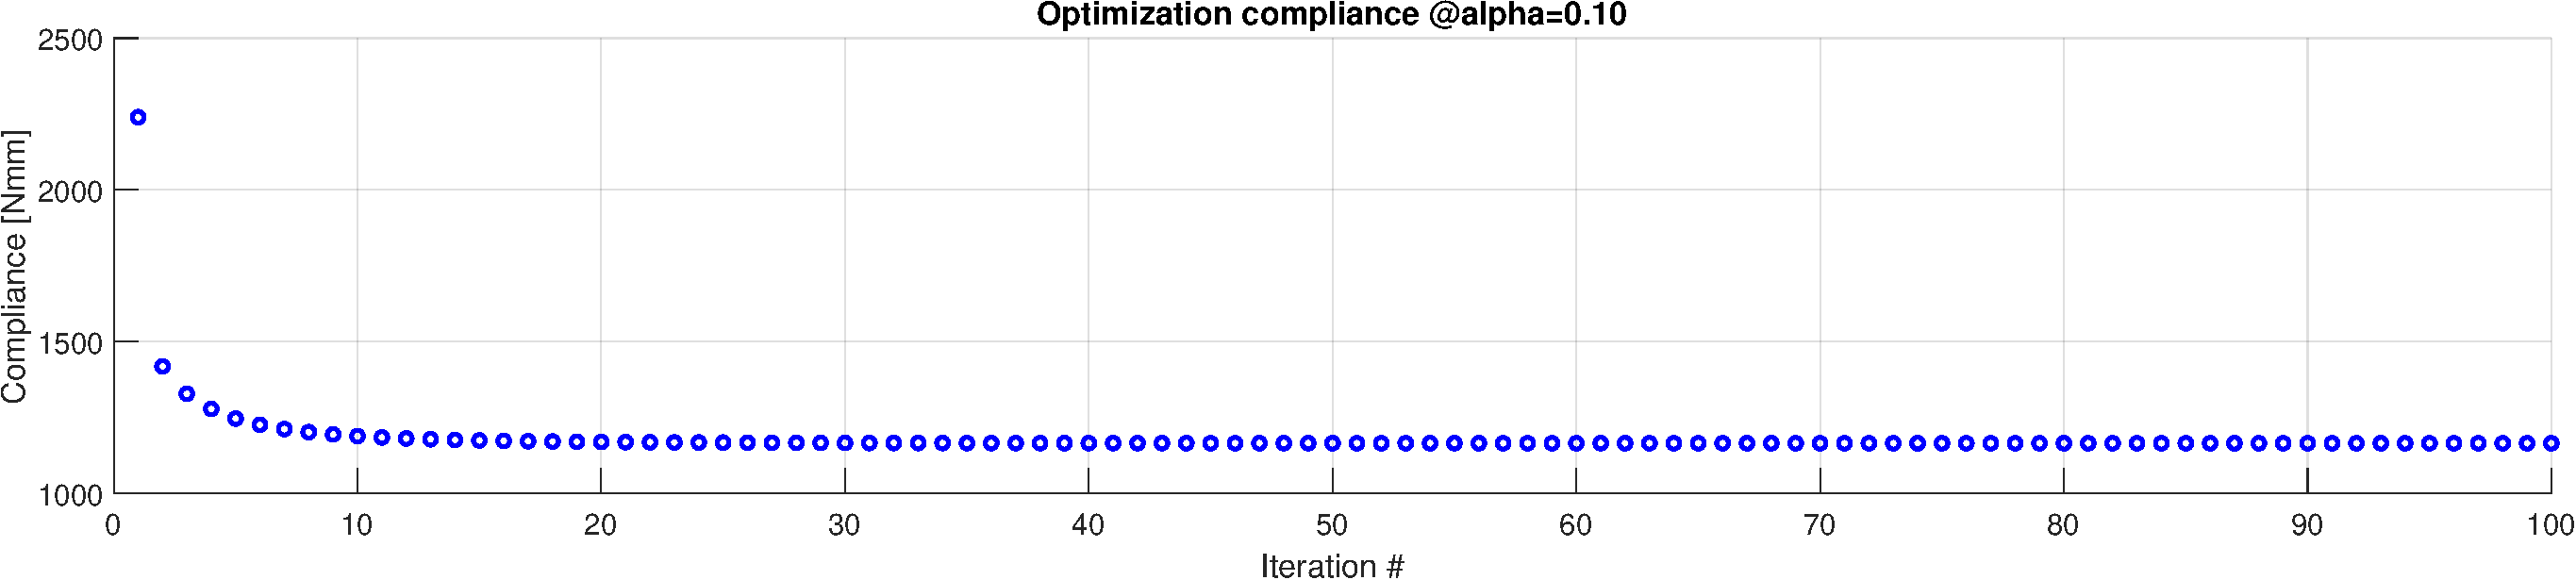
\includegraphics[width=1\textwidth]{img/MATLAB/motorcycle_frame/compliance_alpha10.pdf}
    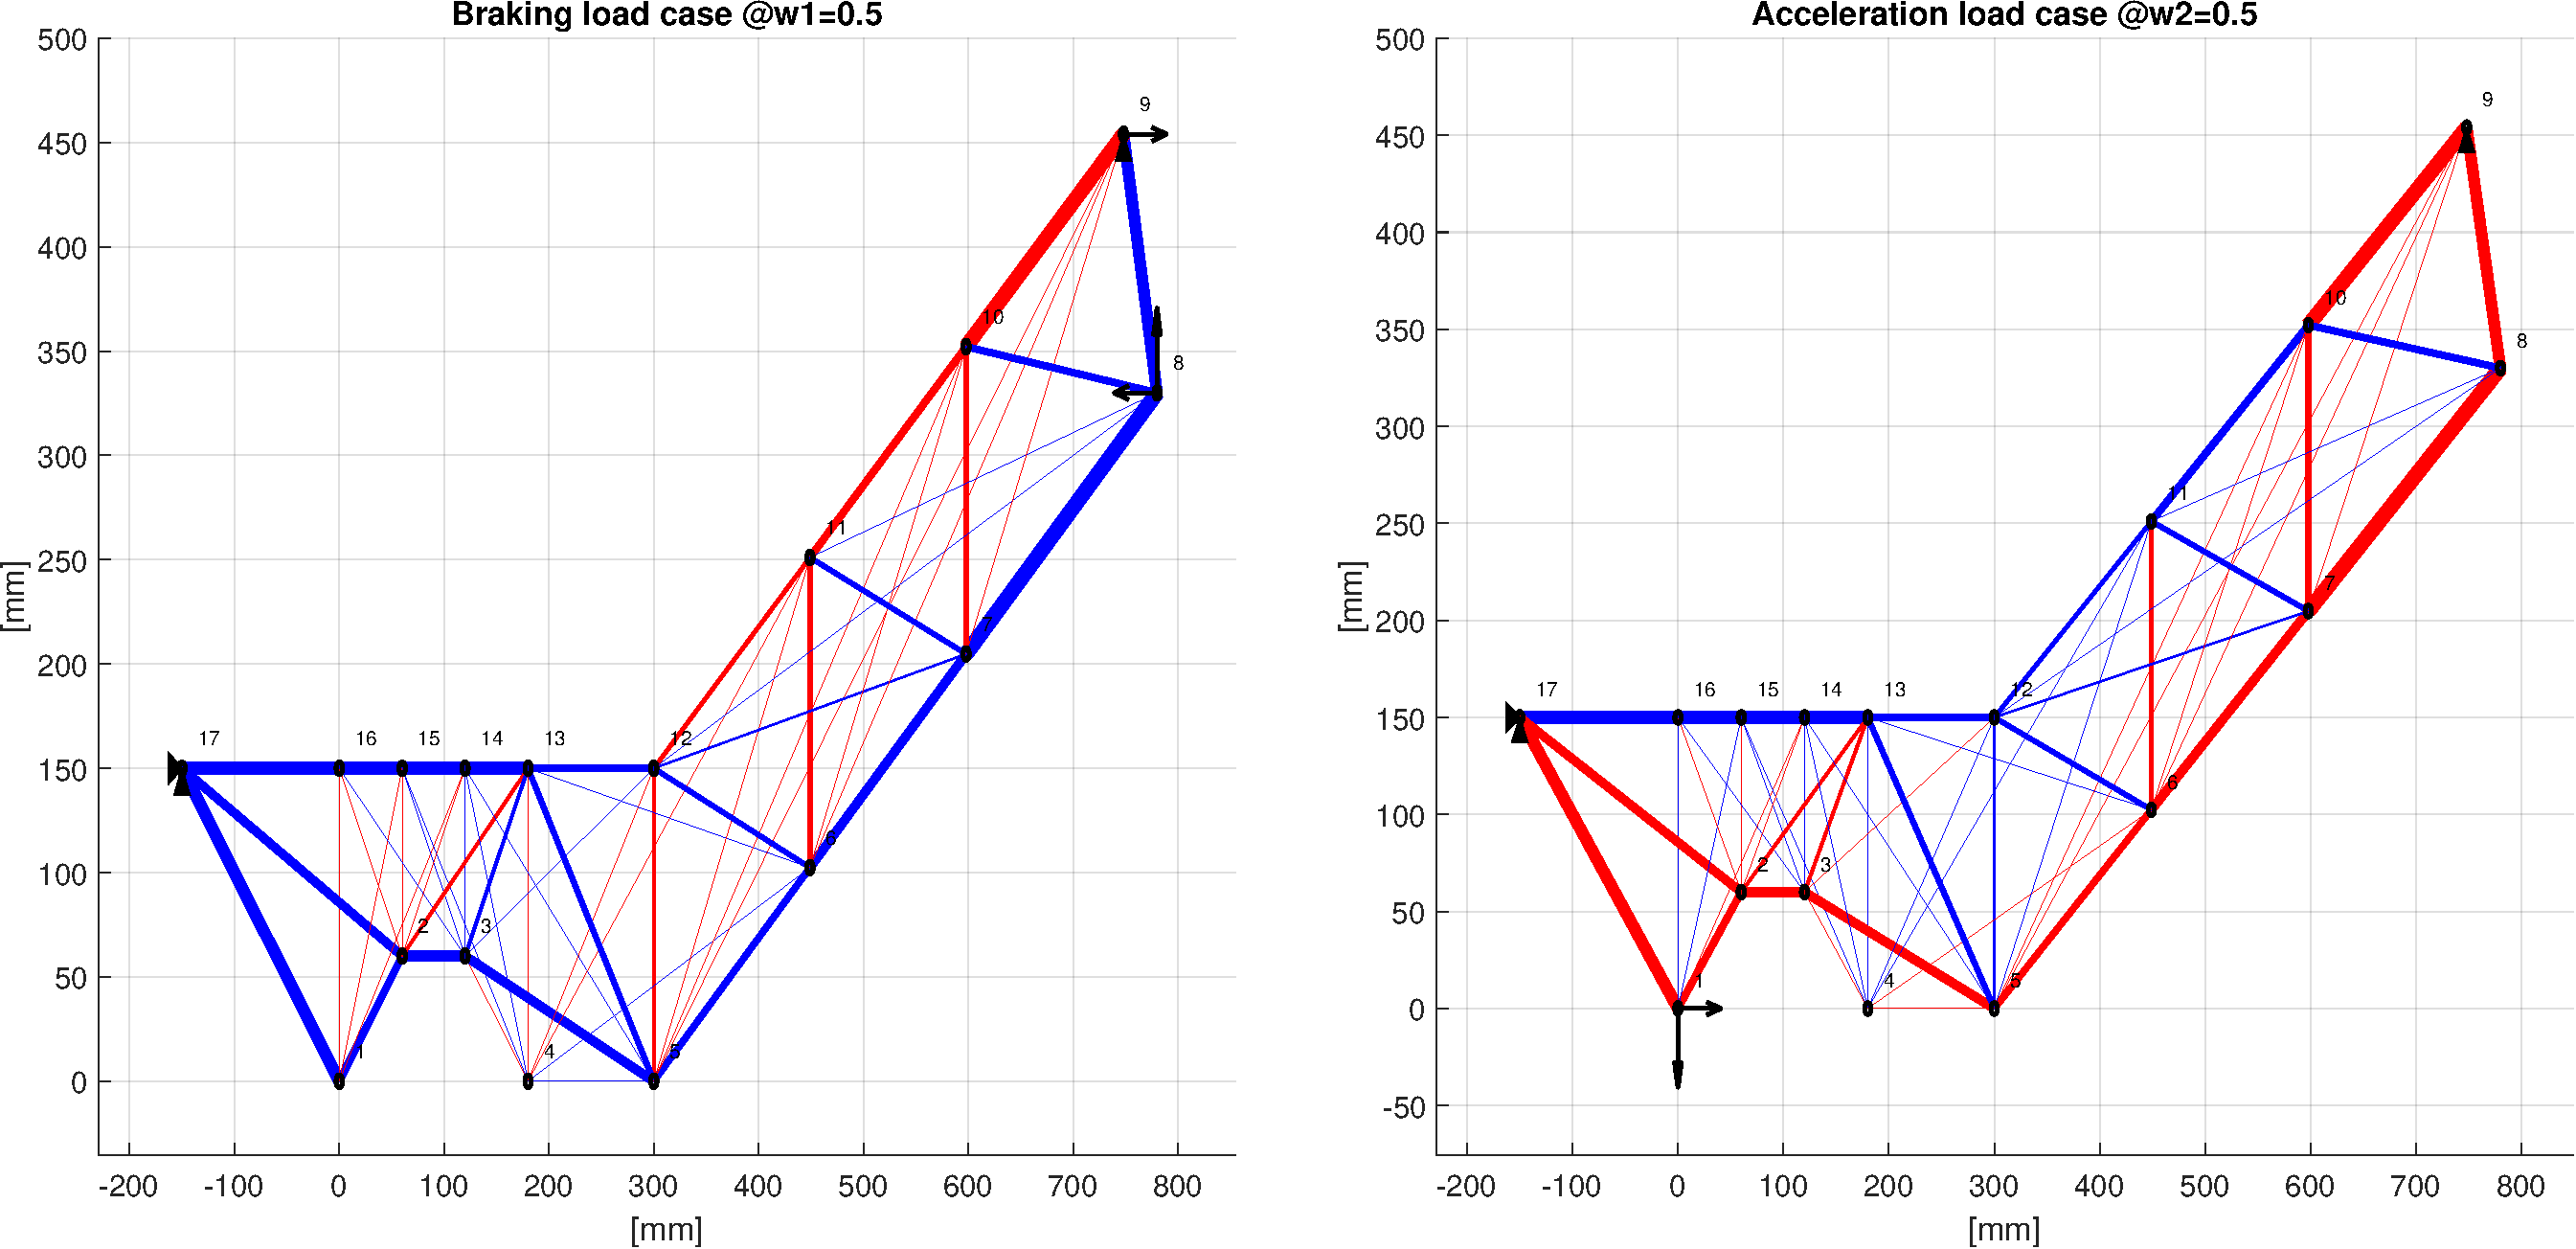
\includegraphics[width=1\textwidth]{img/MATLAB/motorcycle_frame/results_w50.pdf}
    \caption{Optimized motorcycle frame for $w_1 = 0.5$ and $w_2 = 0.5$}
    \label{fig:mf_results_1}
\end{figure}

We now proceed showing the results for different values of $w_1$ and $w_2$.
In particular, we consider the following cases:

\begin{table}[H]
    \centering

    \begin{tabular}{|c|c|c|}
        \hline
        \textbf{Case} & \textbf{$w_1$} & \textbf{$w_2$} \\
        \hline
        1             & 0.0            & 1.0            \\
        2             & 0.2            & 0.8            \\
        3             & 0.8            & 0.2            \\
        4             & 1.0            & 0.0            \\
        \hline
    \end{tabular}

    \caption{Different values of $w_1$ and $w_2$}
    \label{tab:mf_cases}

\end{table}

The results are shown in Figures \ref{fig:mf_results_2}, \ref{fig:mf_results_3}, \ref{fig:mf_results_4} and \ref{fig:mf_results_5}.

\begin{figure}[H]
    \centering
    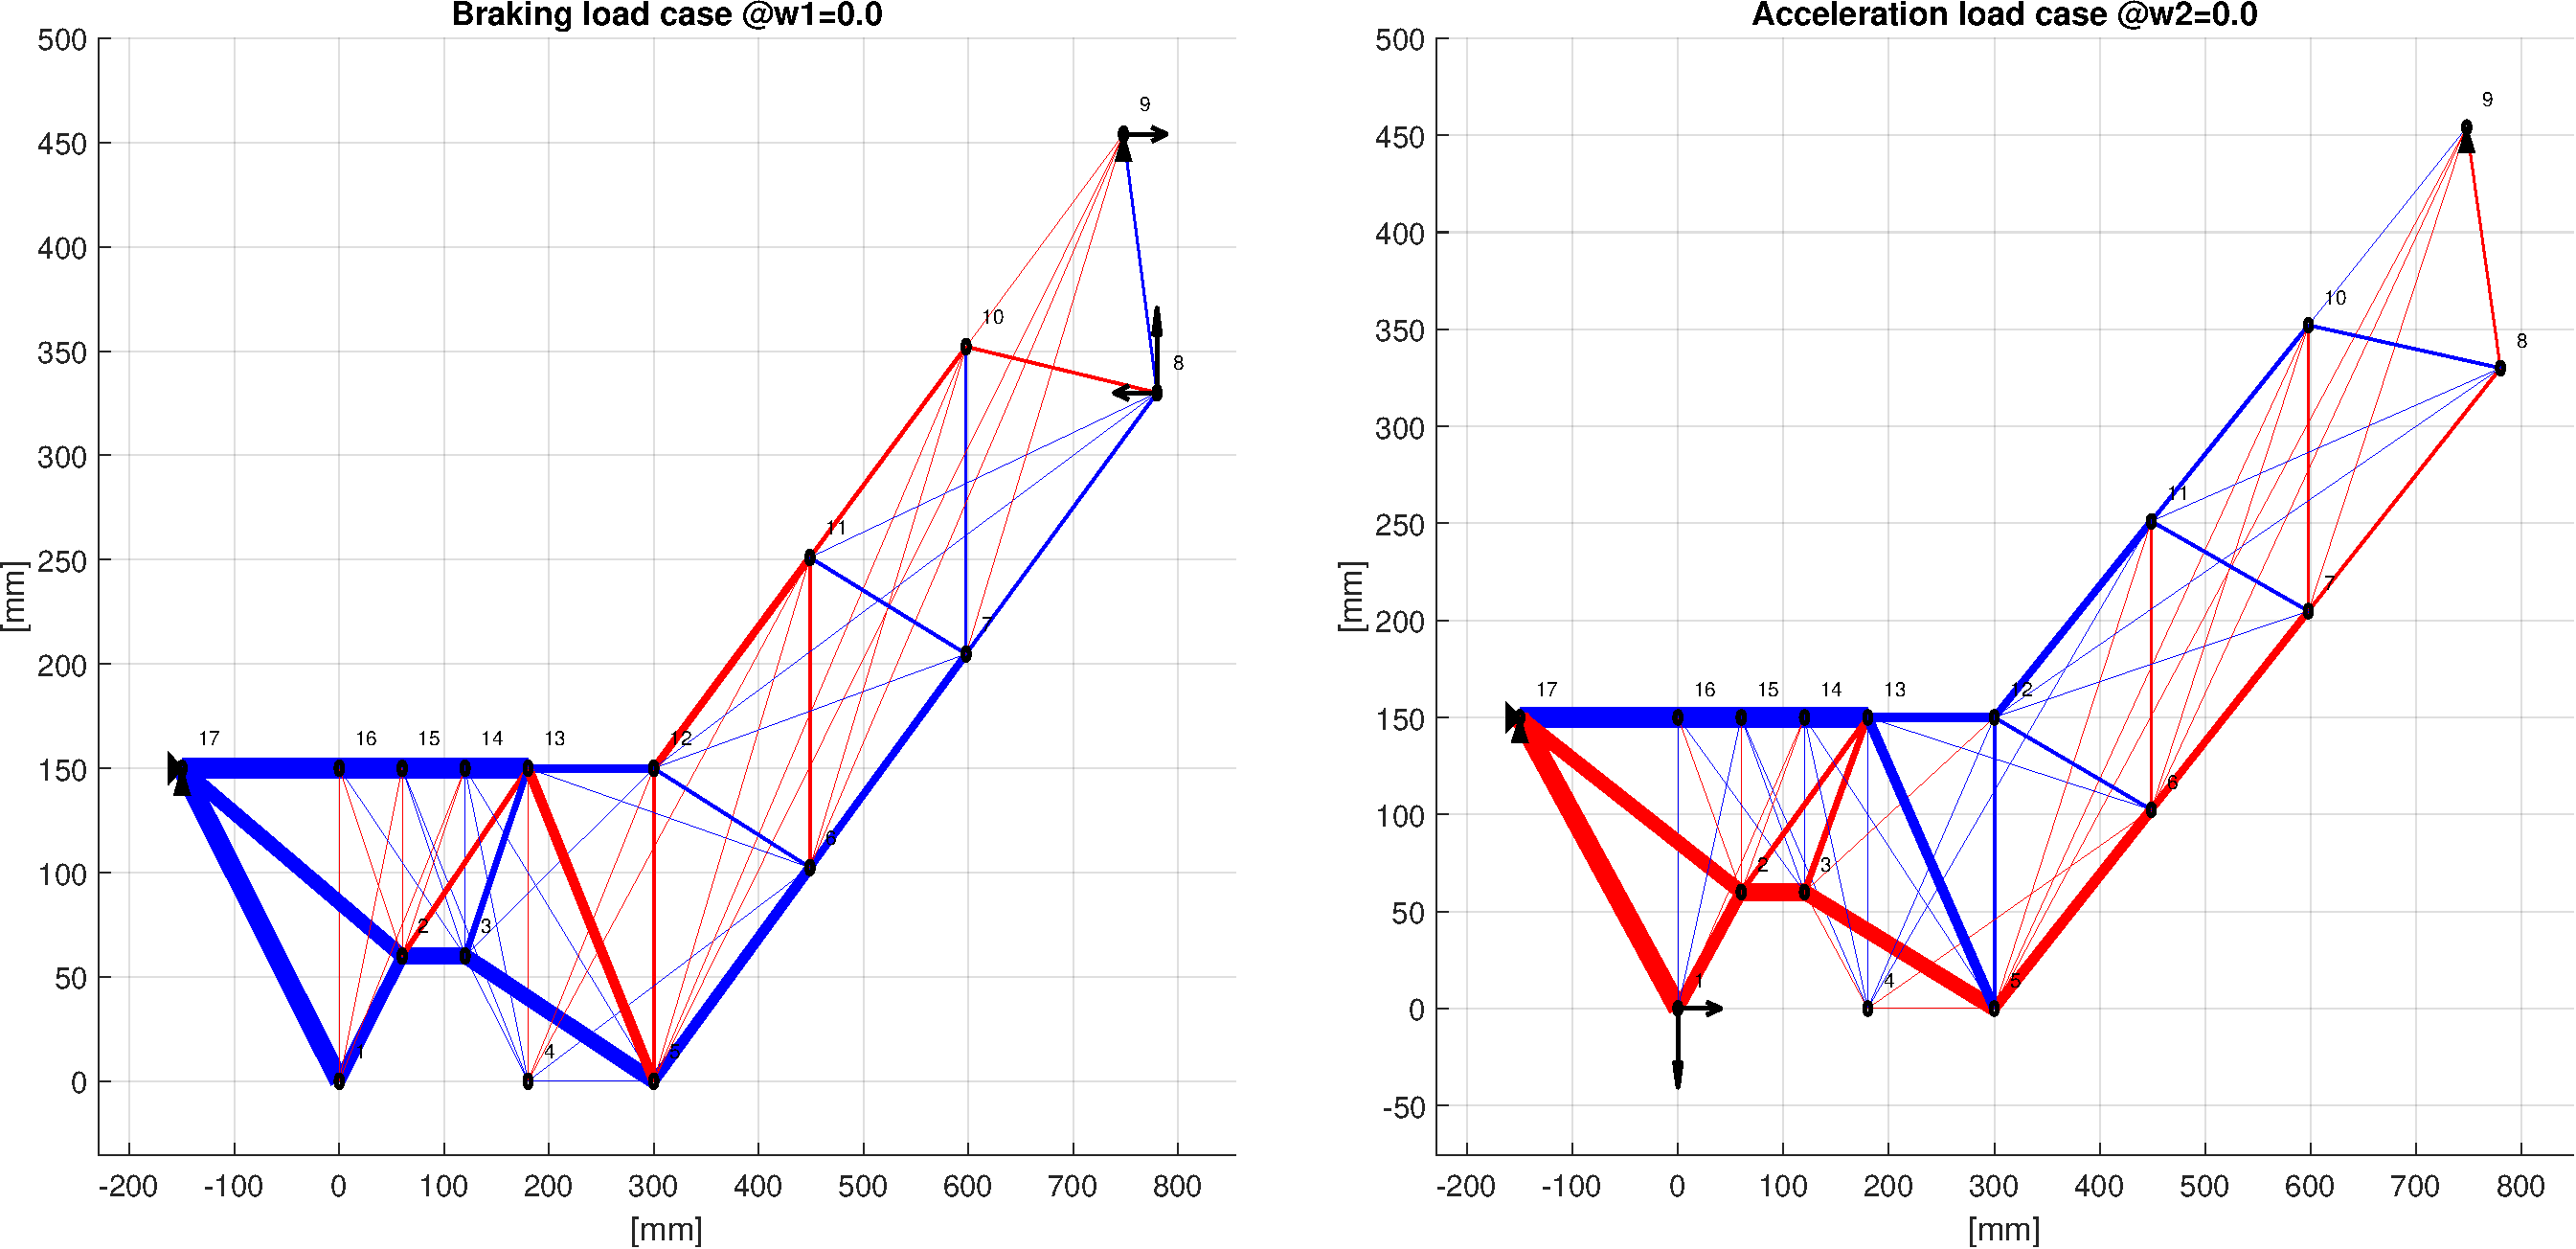
\includegraphics[width=1\textwidth]{img/MATLAB/motorcycle_frame/results_w0.pdf}
    \caption{Optimized motorcycle frame for $w_1 = 0.0$ and $w_2 = 1.0$}
    \label{fig:mf_results_2}
\end{figure}

\begin{figure}[H]
    \centering
    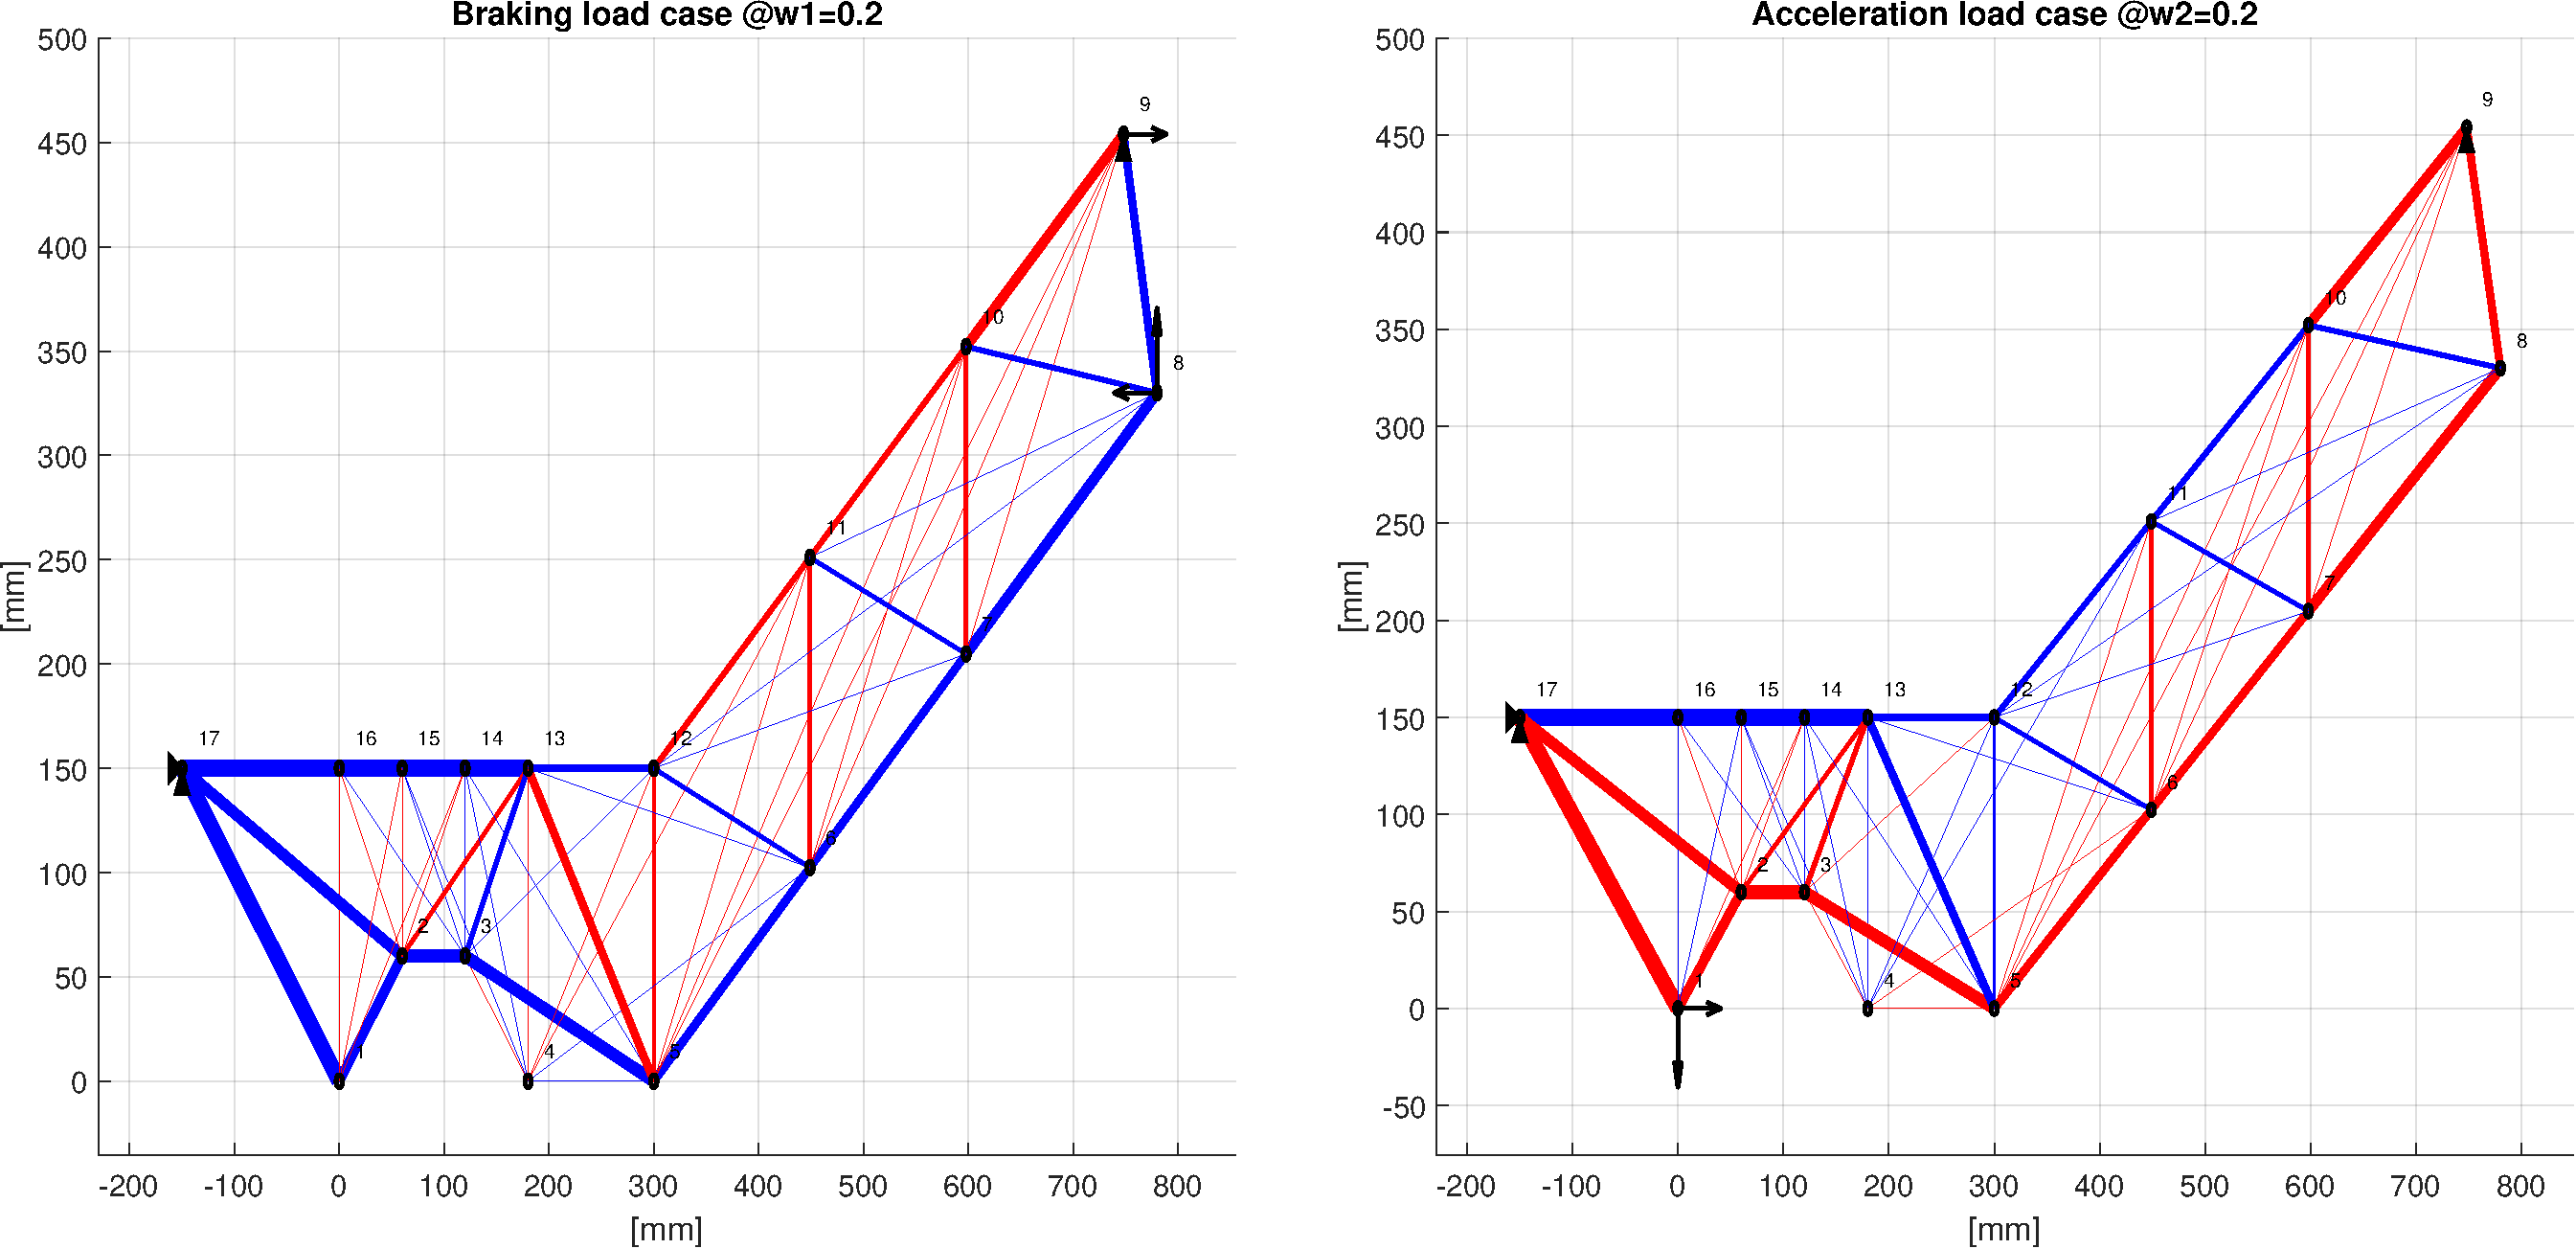
\includegraphics[width=1\textwidth]{img/MATLAB/motorcycle_frame/results_w20.pdf}
    \caption{Optimized motorcycle frame for $w_1 = 0.2$ and $w_2 = 0.8$}
    \label{fig:mf_results_3}
\end{figure}

\begin{figure}[H]
    \centering
    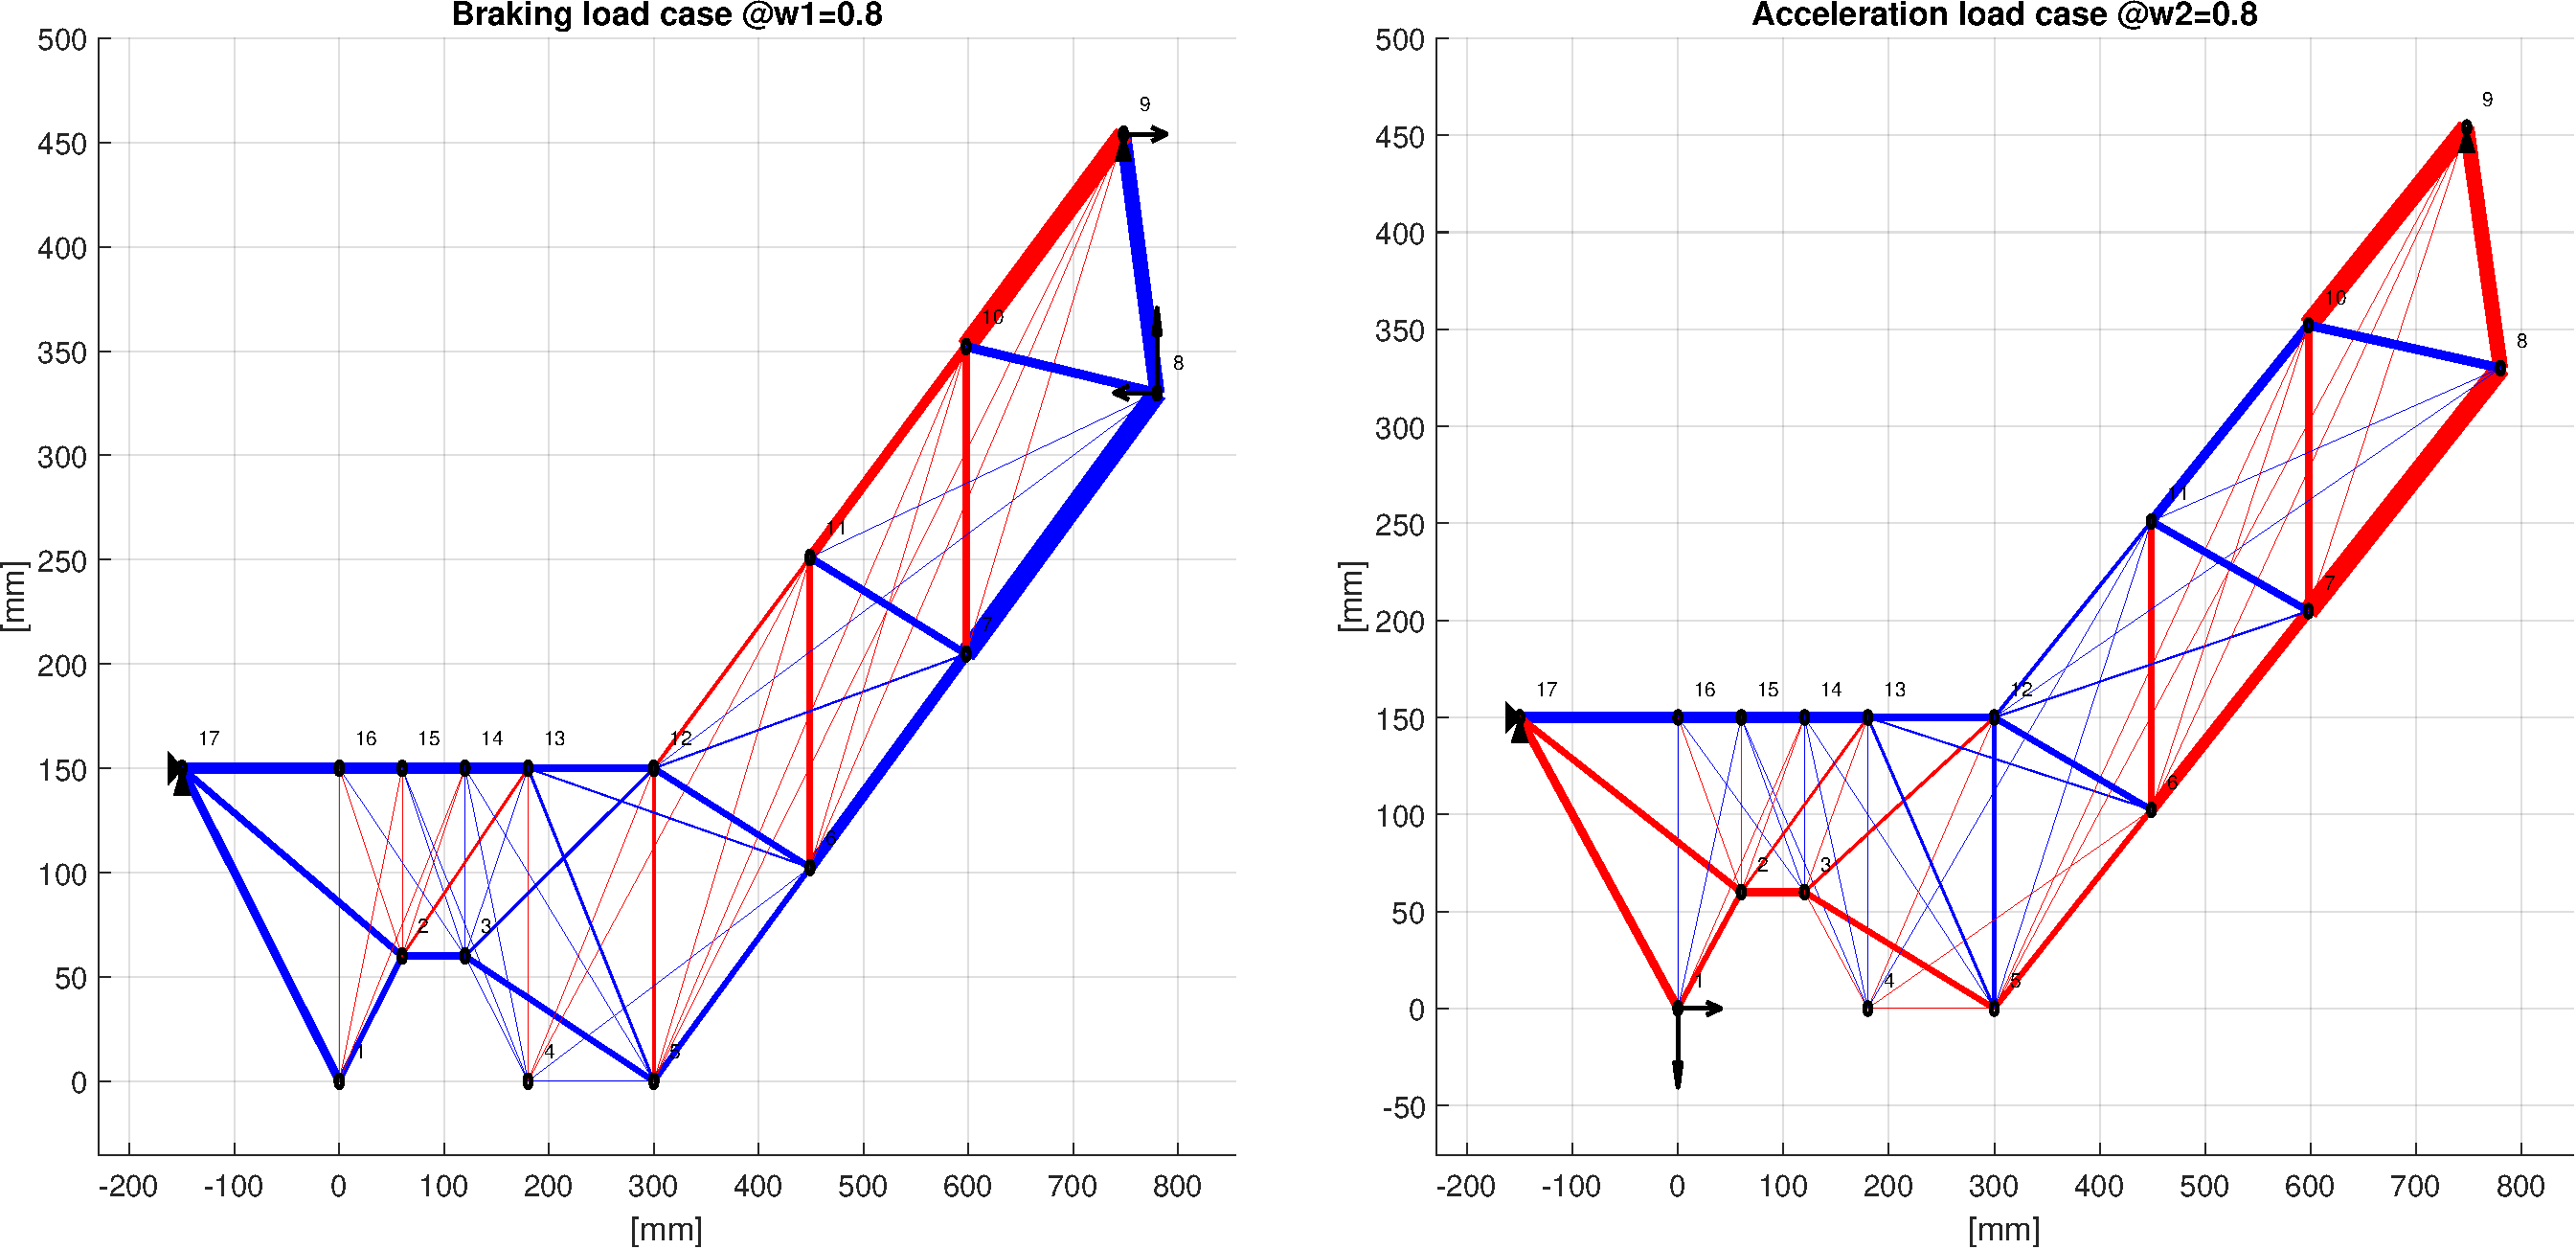
\includegraphics[width=1\textwidth]{img/MATLAB/motorcycle_frame/results_w80.pdf}
    \caption{Optimized motorcycle frame for $w_1 = 0.8$ and $w_2 = 0.2$}
    \label{fig:mf_results_4}
\end{figure}

\begin{figure}[H]
    \centering
    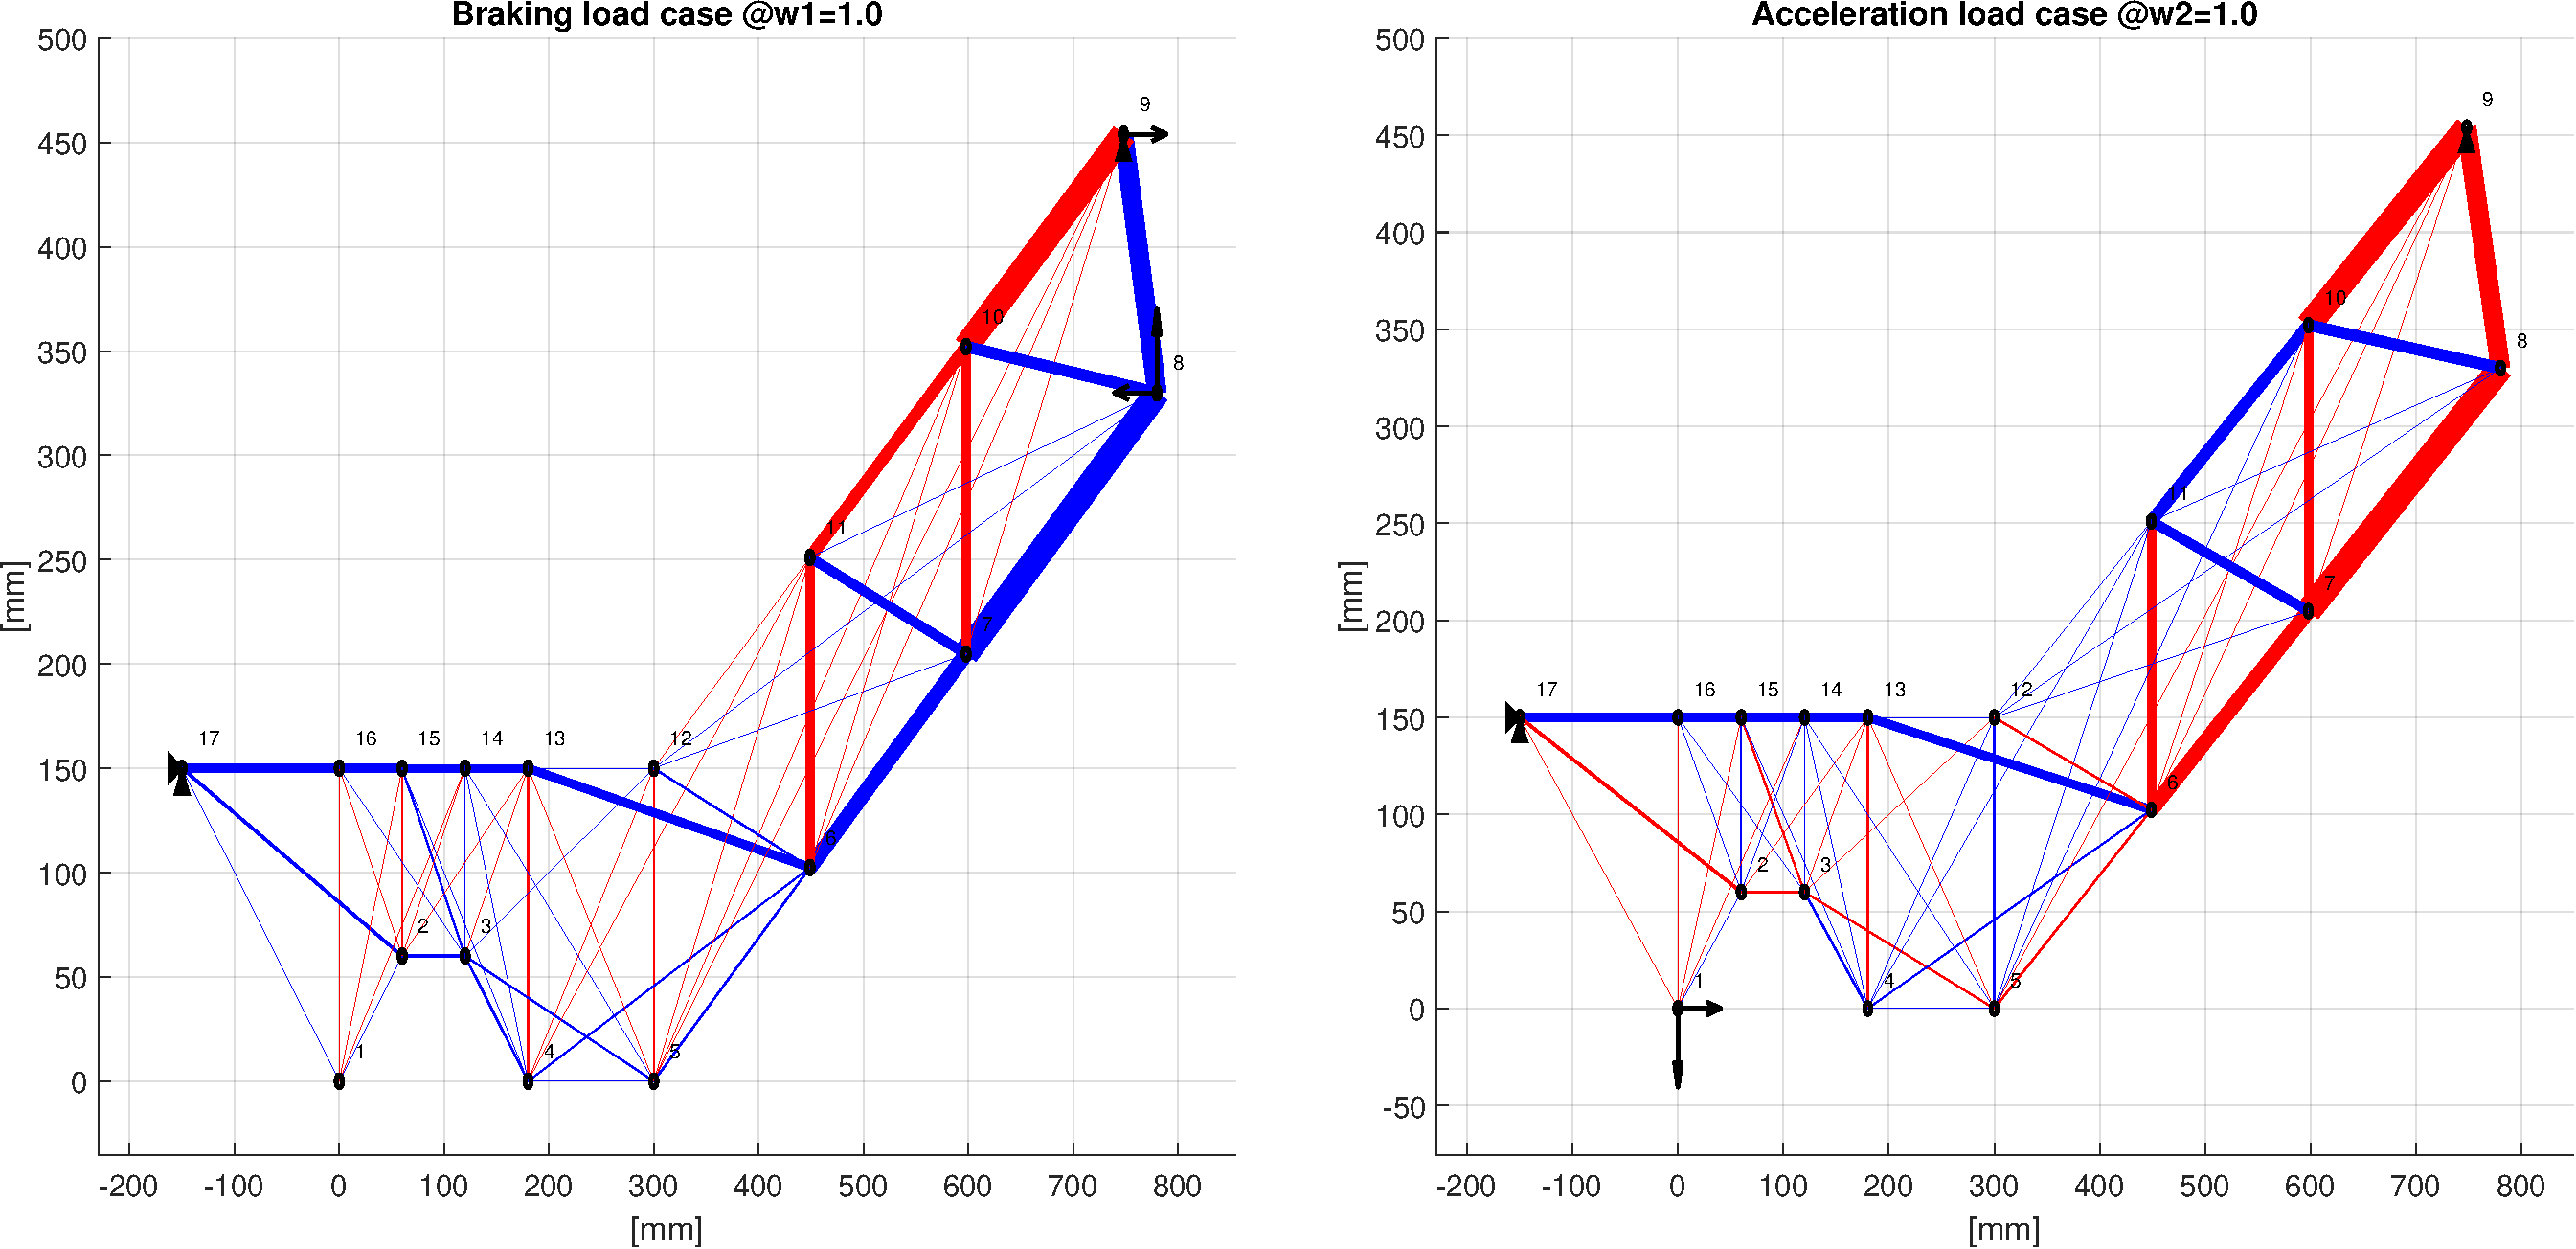
\includegraphics[width=1\textwidth]{img/MATLAB/motorcycle_frame/results_w100.pdf}
    \caption{Optimized motorcycle frame for $w_1 = 1.0$ and $w_2 = 0.0$}
    \label{fig:mf_results_5}
\end{figure}
